\documentclass[12pt, a4paper]{article}

% ============================================================
% Paquetes
% ============================================================
\usepackage[utf8]{inputenc}
\usepackage[T1]{fontenc}
\usepackage[spanish]{babel}
\usepackage{geometry}
\usepackage{amsmath}
\usepackage{amssymb}
\usepackage{graphicx}
\usepackage{booktabs}
\usepackage{array}
\usepackage{xcolor}
\usepackage{hyperref}
\usepackage{parskip}
\usepackage{microtype}
\usepackage{lmodern}

\geometry{
    top    = 2.5cm,
    bottom = 2.5cm,
    left   = 3.0cm,
    right  = 2.5cm,
}

\hypersetup{
    colorlinks = true,
    linkcolor  = blue!70!black,
    urlcolor   = blue!70!black,
    citecolor  = blue!70!black,
}

% ============================================================
% Metadatos del documento
% ============================================================
\title{\textbf{Documentación del Sistema de Calefacción\\con Carga Eléctrica Variable}}
\author{}
\date{}

% ============================================================
\begin{document}
% ============================================================

\maketitle
\tableofcontents
\newpage

% ------------------------------------------------------------
\section{Selección de Resistencias Eléctricas}
% ------------------------------------------------------------

Para el sistema de calefacción se seleccionaron resistencias eléctricas de tipo U con una
potencia nominal de \textbf{1000 W} y voltaje de operación de \textbf{120 V}. Con el fin de
mejorar la eficiencia en la disipación de calor y procurar una distribución uniforme de
temperatura, se estableció que cada resistencia contara con un \textbf{disipador de calor
integrado} de aletas rectangulares, como se muestra en la Figura~\ref{fig:resistencia}.

\begin{figure}[h!]
    \centering
    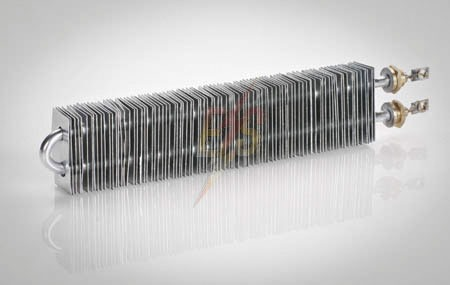
\includegraphics[width=0.5\textwidth]{Imagenes/resistencia.jpeg}
    \caption{Resistencia eléctrica de tipo U con disipador de calor de aletas rectangulares.}
    \label{fig:resistencia}
\end{figure}

Se definió como temperatura máxima de operación \textbf{200\,°C}, valor indicado por el
fabricante, con el propósito de garantizar la integridad del componente y asegurar condiciones
seguras de funcionamiento. La ficha técnica del material de la resistencia se encuentra en la
carpeta \texttt{Fichas Tecnicas} con el nombre \texttt{Ficha Tecnica Material Resistencia.pdf}.

% ------------------------------------------------------------
\section{Análisis Térmico: Convección Forzada}
% ------------------------------------------------------------

Para determinar la potencia máxima que puede disipar el sistema antes de que la resistencia
alcance los 200\,°C, se realizó un análisis de \textbf{transferencia de calor por convección
forzada externa} sobre un banco de tubos escalonado. Los cálculos se encuentran en la carpeta \texttt{Calculos} con el nombre \texttt{Calculos\_Ventilador.py}.

\subsection{Modelado de la resistencia}

Dado que la resistencia tiene geometría cilíndrica, se empleó una \textbf{sección transversal
rectangular equivalente} de igual perímetro que el cilindro original (misma área superficial
lateral). Esto permite aplicar las correlaciones del banco de tubos con mayor facilidad,
siguiendo las suposiciones descritas en el \textbf{Capítulo~3.6} del libro \textit{Heat and
Mass Transfer: Fundamentals \& Applications} (Yunus A. Çengel, 6.\textsuperscript{a} edición).

\subsection{Modelado del disipador de calor}

El disipador se modeló con \textbf{4 aletas rectangulares por sección transversal}, orientadas
en las cuatro direcciones principales. Cada aleta se extiende 15\,mm desde el centro del tubo,
con un espesor de 1\,mm y una separación entre planos de aletas de 2\,mm. Se definieron,
además, \textbf{zonas sin aletas} en los extremos del tubo:

\begin{itemize}
    \item \textbf{Zona inferior:} 45\,mm (zona de conexión eléctrica).
    \item \textbf{Zona superior:} 15\,mm (extremo de la pata de la U).
\end{itemize}

Todas estas medidas fueron tomadas con un calibrador al momento de recibir el producto.

La eficiencia de cada aleta se calculó mediante la expresión:

\begin{equation}
    \eta_{\text{aleta}} = \frac{\tanh(m L_c)}{m L_c},
    \qquad
    m = \sqrt{\frac{2h}{k_{\text{aleta}} \cdot t}}
    \label{eq:eta_aleta}
\end{equation}

donde $L_c$ es la longitud corregida que incorpora el efecto de la punta de la aleta
($L_c = L + t/2$), según la \textbf{Tabla 3-3 y la Ecuación~3-77} de Çengel.

El área efectiva total por tubo se calculó como:

\begin{equation}
    A_{\text{eff}} = A_{\text{libre}} + \eta_{\text{aleta}} \cdot A_{\text{aletas}}
    \label{eq:A_eff}
\end{equation}

(Ecuación~3-81, Çengel).

\subsection{Correlaciones del banco de tubos}

Para el coeficiente de convección $h$, se utilizaron las \textbf{correlaciones de Zukauskas
para flujo externo en bancos de tubos escalonados} (Tabla~7-2 y Tabla~7-3, Çengel,
Capítulo~7, Sección~7.4). El número de Nusselt promedio, corregido por el factor de
configuración $F$ (para $N_L < 16$ filas), se empleó para determinar $h$, y a partir de este
se calculó la potencia disipada por el sistema completo.

% ------------------------------------------------------------
\section{Configuraciones Evaluadas}
% ------------------------------------------------------------

Se analizaron \textbf{6 resistencias de tipo U} (12 tubos en total), cada una con potencia
nominal de 1000\,W, para un total de \textbf{6000\,W} a disipar. Se evaluaron dos
configuraciones de arreglo, descritas en la Tabla~\ref{tab:configs}.

\begin{table}[h!]
    \centering
    \caption{Configuraciones de arreglo evaluadas.}
    \label{tab:configs}
    \begin{tabular}{>{\centering\arraybackslash}m{2.2cm}
                    >{\centering\arraybackslash}m{2.2cm}
                    >{\centering\arraybackslash}m{3cm}
                    m{4.8cm}}
        \toprule
        \textbf{Configuración} & \textbf{Filas ($N_L$)} & \textbf{Tubos por fila ($N_T$)} & \textbf{Descripción} \\
        \midrule
        A & 3 & 4 & 2 resistencias por fila \\
        B & 6 & 2 & 1 resistencia por fila  \\
        \bottomrule
    \end{tabular}
\end{table}

Para ambas configuraciones se fijó el \textbf{paso transversal} $S_T = 3\,\text{cm}$ y se
realizó un \textbf{estudio paramétrico} variando el paso longitudinal $S_L$ entre 4\,cm y
10\,cm, con incrementos de 1\,cm, con el objetivo de determinar la velocidad de aire mínima
requerida y la caída de presión asociada.

% ------------------------------------------------------------
\section{Conclusiones del Análisis Térmico}
% ------------------------------------------------------------

Gracias a la incorporación del disipador de calor, el área efectiva de transferencia de calor
aumentó significativamente con respecto a la superficie desnuda del tubo. Como resultado, se
obtuvo que la \textbf{velocidad de aire requerida para alcanzar los 200\,°C en la superficie
de la resistencia es considerablemente baja}, por debajo de los rangos típicos de operación
de ventiladores comerciales.

En consecuencia, bajo condiciones normales de operación con los ventiladores seleccionados,
\textbf{la temperatura superficial de la resistencia no debería alcanzar el límite máximo de
200\,°C}, lo cual proporciona un margen de seguridad adecuado para el sistema. La ficha
técnica de los ventiladores se encuentra en la carpeta \texttt{Fichas Tecnicas} con el nombre
\texttt{Ficha Tecnica Ventiladores.pdf}.

La \textbf{configuración óptima} (mínima potencia del ventilador) fue identificada a partir del
estudio paramétrico, evaluando simultáneamente la velocidad requerida, la caída de presión
$\Delta P$ y la potencia del ventilador $\dot{W}_{\text{fan}} = \dot{V} \cdot \Delta P$.
Después del estudio paramétrico se determinó que la configuración óptima es la
\textbf{Configuración B} con un paso longitudinal de 4\,cm, como se muestra en la
Figura~\ref{fig:dist_optima}.

\begin{figure}[h!]
    \centering
    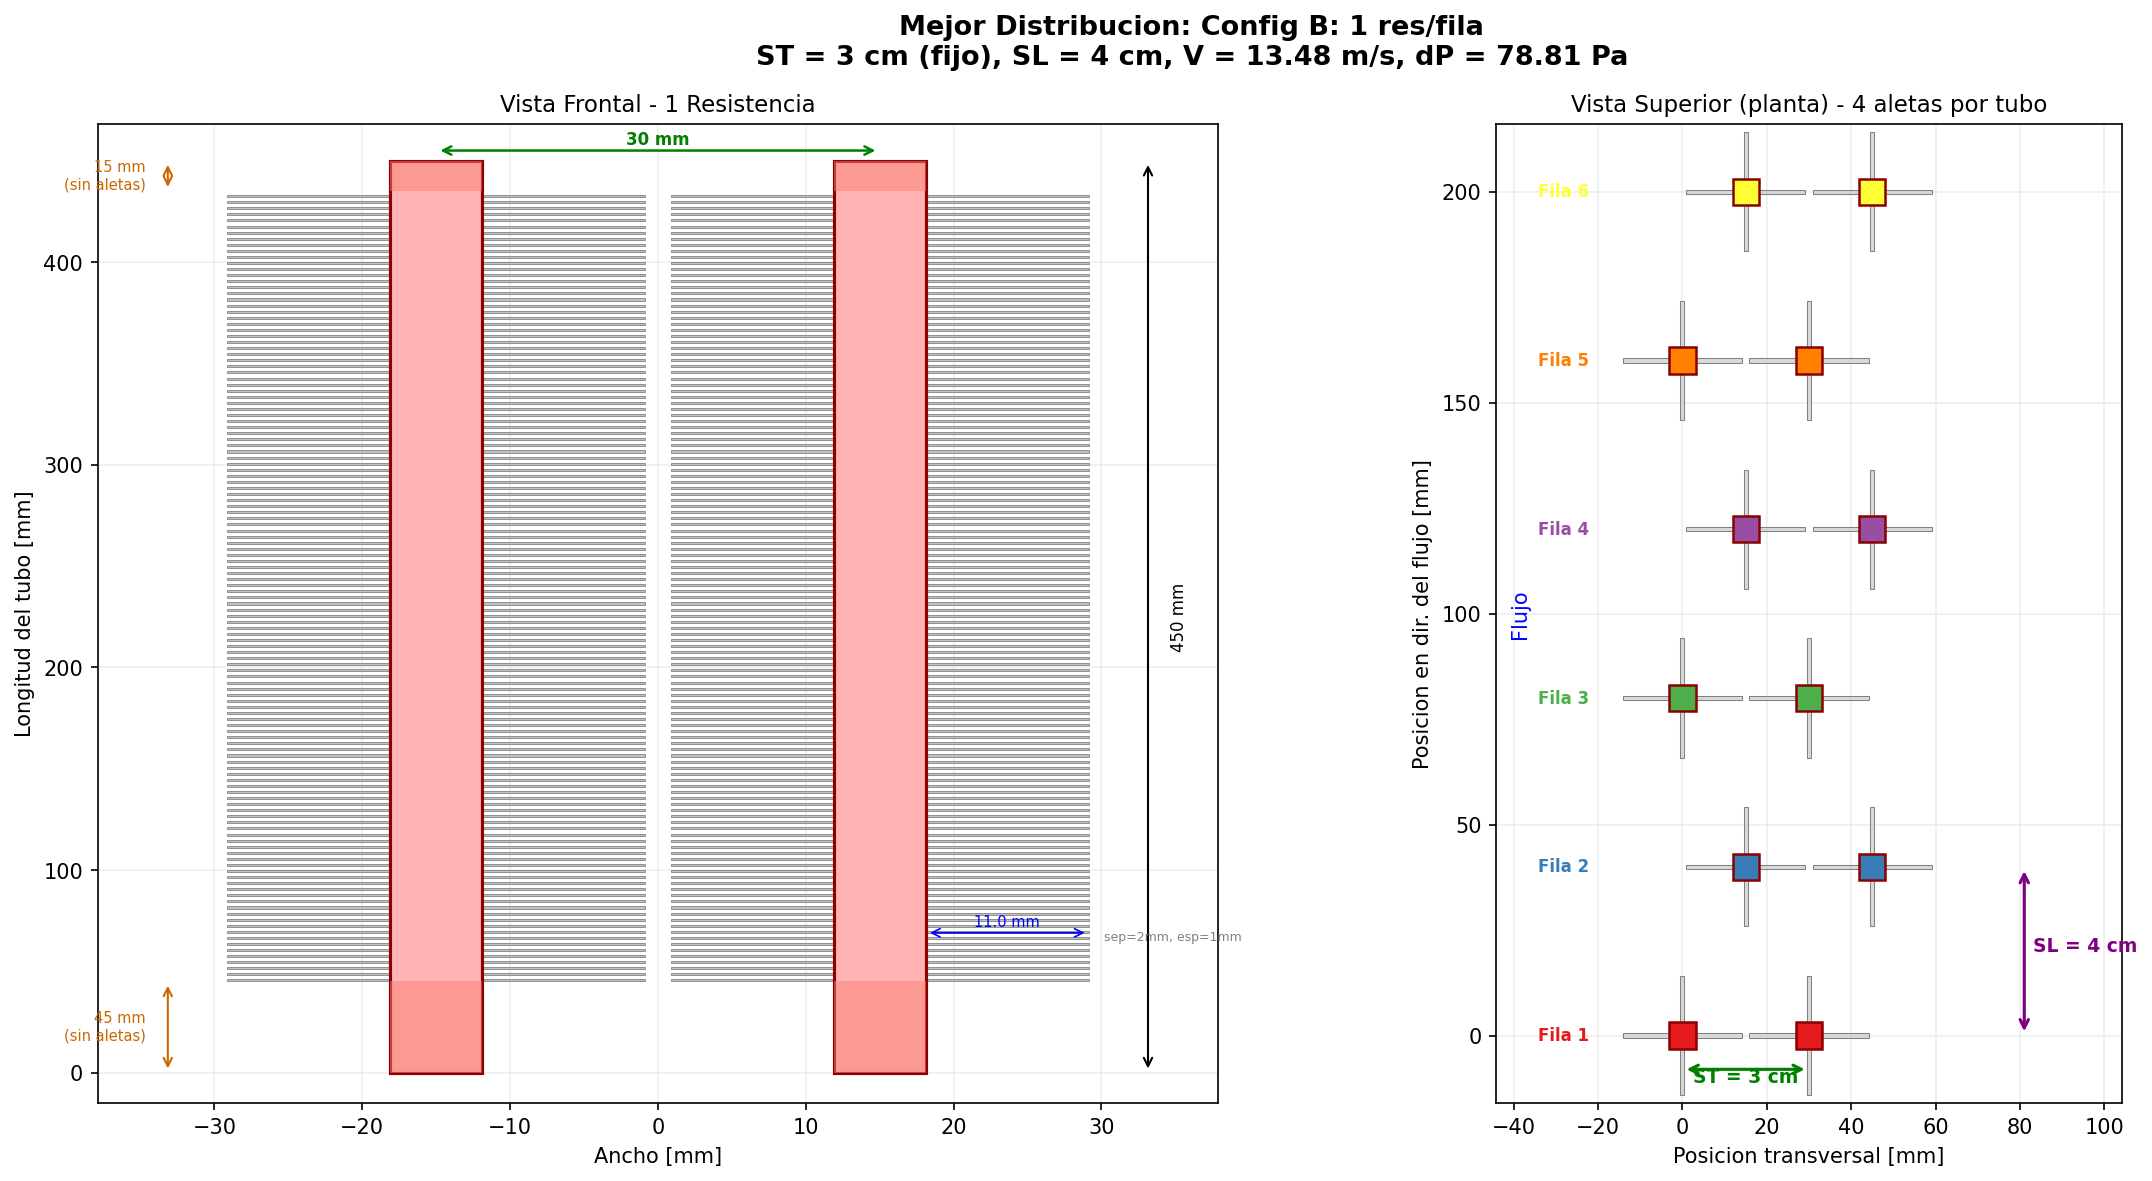
\includegraphics[width=0.85\textwidth]{Imagenes/distribucion_optima.png}
    \caption{Distribución óptima del banco de tubos (Configuración B, $S_L = 4\,\text{cm}$).}
    \label{fig:dist_optima}
\end{figure}

% ------------------------------------------------------------
\section{Diseño Mecánico: Caja Contenedora}
% ------------------------------------------------------------

Con las resistencias y ventiladores seleccionados, se procedió al diseño del \textbf{modelo
CAD de la caja} que alberga el sistema completo (disponible en la carpeta
\texttt{Modelos CAD} con el nombre \texttt{Caja.step}). El diseño contempla los siguientes
aspectos:

\begin{itemize}
    \item \textbf{Integración de componentes:} Alojamiento estructurado para las 6 resistencias
    en U y los ventiladores.

    \item \textbf{Material aislante interior:} Dado que el sistema estará en contacto frecuente
    con estudiantes, se incorporó un \textbf{revestimiento de material aislante térmico} en el
    interior de la caja para prevenir quemaduras por contacto accidental con superficies
    calientes. La ficha técnica se encuentra en \texttt{Fichas Tecnicas/Ficha Tecnica Material
    Aislante.pdf}.

    \item \textbf{Seguridad eléctrica:} Se prevé el uso de materiales resistentes a altas
    temperaturas para recubrir los cables en las zonas expuestas al calor generado por las
    resistencias. La ficha técnica se encuentra en \texttt{Fichas Tecnicas/Ficha Tecnica
    Cable.pdf}.
\end{itemize}

% ------------------------------------------------------------
\section{Pruebas de Funcionamiento}
% ------------------------------------------------------------

Se realizó una primera prueba experimental para verificar las temperaturas que alcanzan los distintos componentes de la máquina bajo condiciones reales de operación. El sistema fue operado a su máxima capacidad de \textbf{6\,kW} durante un período continuo de \textbf{10 minutos}. 

Las temperaturas registradas al finalizar la prueba fueron las siguientes:

\begin{itemize}
    \item \textbf{Resistencia trasera:} 168\,°C
    \item \textbf{Componentes eléctricos:} 46\,°C
    \item \textbf{Carcasa:} 45\,°C
    \item \textbf{Conectores a las resistencias:} 39\,°C
    \item \textbf{Cables:} 36\,°C
\end{itemize}

Estos resultados confirman que la temperatura de la resistencia (168\,°C) se mantiene por debajo del límite de diseño (200\,°C), tal como se predijo en el análisis térmico. Asimismo, las temperaturas de la carcasa, los componentes eléctricos y los cables se encuentran en rangos seguros para la operación y manipulación del equipo. Aunque se esperaba que la temperatura de los componentes eléctricos fuera menor, por lo que se va a contemplar el uso de material aislante térmico entre las resistencias y la carcasa para reducir la temperatura con el objetivo de evitar quemaduras por contacto accidental.

% ------------------------------------------------------------
\section{Referencias}
% ------------------------------------------------------------

\begin{itemize}
    \item Çengel, Y.\,A., \& Ghajar, A.\,J. (2020). \textit{Heat and Mass Transfer:
    Fundamentals \& Applications} (6.\textsuperscript{a}\,ed.). McGraw-Hill Education.
    \begin{itemize}
        \item Capítulo~3, Sección~3.6: Eficiencia de aletas rectangulares\\
              (Tabla~3-3, Ec.~3-72, Ec.~3-77, Ec.~3-81).
        \item Capítulo~7, Sección~7.4: Convección forzada externa en bancos de tubos\\
              (Tabla~7-2, Tabla~7-3, Fig.~7-27b, Ec.~7-40, 7-41, 7-45).
    \end{itemize}
\end{itemize}

\end{document}
